\documentclass[11pt,a4paper]{article}

% Essential Packages
\usepackage[utf8]{inputenc}
\usepackage[margin=1in]{geometry}
\usepackage{amsmath,amssymb,amsfonts,bm}
\usepackage{graphicx}
\usepackage{booktabs}
\usepackage{xcolor}
\usepackage{tikz}
\usetikzlibrary{shapes.geometric, arrows.meta, positioning, calc, backgrounds}
\usepackage{hyperref}
\usepackage{float}
\usepackage{enumitem}
\usepackage{tcolorbox}

% Colors
\definecolor{primaryblue}{RGB}{33, 102, 172}
\definecolor{accentorange}{RGB}{214, 96, 77}
\definecolor{darkgreen}{RGB}{39, 100, 25}
\definecolor{lightgraybg}{RGB}{248, 249, 250}
\definecolor{boxborder}{RGB}{209, 213, 219}

% Hyperref setup
\hypersetup{
    colorlinks=true,
    linkcolor=primaryblue,
    citecolor=primaryblue,
    urlcolor=primaryblue
}

% Custom Callout Box for Discussion Points
\newtcolorbox{discussionbox}[1]{
    colback=lightgraybg,
    colframe=boxborder,
    fonttitle=\bfseries\color{primaryblue},
    title=#1,
    boxrule=1pt,
    arc=3pt,
    left=6pt,
    right=6pt,
    top=6pt,
    bottom=6pt
}

% Title and Metadata
\title{\textbf{\LARGE Gradient Descent as Solver vs OR Algos (Simplex)}\\[0.3em]
\large A Systematic Investigation into KKT-Informed Neural Networks for Linear Programming}
\author{\textbf{BTech Project Technical Progress Report} \\ Supervisor Discussion and Formulation Synthesis}
\date{September 2026}

\begin{document}

\maketitle

\begin{abstract}
This report outlines the technical progression, architectural iterations, failure modes, and mathematical insights gained while exploring whether Physics-Informed and KKT-Informed Neural Networks (KINNs) trained via gradient descent can serve as general-purpose linear programming solvers. Starting from standard physics-informed baseline architectures in recent literature, we document five distinct iterations. For each iteration, we detail the specific failure mechanisms, mathematical loss formulations, architectural adjustments, and theoretical underpinnings. Finally, by comparing the continuous nature of neural gradient descent with the discrete, combinatorial nature of traditional Operations Research (OR) algorithms (such as Simplex and Interior Point methods), we re-evaluate our fundamental premise and reformulate our core research question from \textit{``Use KINNs as a solver''} to \textit{\textbf{``Can KINNs be used as a solver?''}}
\end{abstract}

\vspace{0.5em}
\hrule
\vspace{1.5em}

% ----------------------------------------------------------------------
\section{Initial Problem Statement and Motivation}
% ----------------------------------------------------------------------

\subsection{The Starting Premise}
When this project began, the objective appeared to be a direct application of Deep Learning (DL) to Mathematical Programming:
\begin{itemize}[leftmargin=1.5em, itemsep=2pt]
    \item \textbf{Initial Idea:} Formulate the Karush-Kuhn-Tucker (KKT) optimality conditions of a Linear Program (LP) as an unconstrained composite loss function.
    \item \textbf{Optimization Vehicle:} Use standard deep neural networks parameterized by weights $\Theta$ and optimize them end-to-end using first-order gradient descent (Adam / SGD).
    \item \textbf{Target Outcome:} Replace traditional Operations Research (OR) solvers with a continuous, GPU-accelerated neural solver that predicts optimal primal solutions $x^*$ and dual shadow prices $\lambda^*$ in a single training run.
\end{itemize}

\subsection{Standard Form of the Linear Program}
Throughout this document, we consider standard inequality-form linear programs:
\begin{equation}
    \min_{x \in \mathbb{R}^n} \quad c^T x \quad \text{subject to} \quad G x \le h, \quad x \ge 0
\end{equation}
where $c \in \mathbb{R}^n$, $G \in \mathbb{R}^{m \times n}$, and $h \in \mathbb{R}^m$. The associated first-order KKT optimality conditions are:
\begin{enumerate}[leftmargin=1.8em, itemsep=2pt]
    \item \textbf{Primal Feasibility:} $G x - h \le 0$ and $x \ge 0$.
    \item \textbf{Dual Feasibility:} $\lambda \ge 0$.
    \item \textbf{Stationarity:} $c + G^T \lambda - \mu = 0$ (where $\mu \ge 0$ is the multiplier for $x \ge 0$).
    \item \textbf{Complementary Slackness:} $\lambda_i (G x - h)_i = 0$ for all $i \in \{1, \dots, m\}$ and $\mu_j x_j = 0$ for all $j \in \{1, \dots, n\}$.
\end{enumerate}

\subsection{Purpose of this Document}
This document is prepared specifically for technical discussion with the project supervisor. Rather than presenting only positive final results, it systematically documents every failure mode encountered, the mathematical reason for the failure, the counter-measure introduced, and the resulting insights.

\vspace{1em}
\hrule
\vspace{1.5em}

% ----------------------------------------------------------------------
\section{Iteration 1: Baseline Coupled PINN / Unnormalized KKT Loss}
% ----------------------------------------------------------------------

\subsection{Literature Baseline and Paper Description}
The first concept followed baseline formulations from literature on Physics-Informed Neural Networks (PINNs) applied to constrained optimization. The standard recipe in these papers is:
\begin{itemize}[leftmargin=1.5em, itemsep=2pt]
    \item Feed a fixed dummy input (such as a constant vector of ones $\mathbf{1}$) into a Multi-Layer Perceptron (MLP).
    \item Use a single shared neural network whose output layer is split to predict both primal variables $\hat{x}$ and dual variables $\hat{\lambda}$.
    \item Formulate an unweighted or fixed-weight penalty loss summing the squared violations of the KKT conditions.
\end{itemize}

\subsection{Problems Faced in Iteration 1 (Point-Wise Breakdown)}
When tested on the Netlib benchmark suite, this initial concept failed severely:
\begin{itemize}[leftmargin=1.5em, itemsep=3pt]
    \item \textbf{Destructive Gradient Interference (Coupled MLP):} Primal minimization requires gradients driven by cost vector $c$, while dual stationarity requires gradients driven by $G^T \lambda$. Sharing hidden layers forced backpropagation to add these opposing gradient vectors together, resulting in near-zero effective updates:
    \begin{equation}
        \nabla_W \mathcal{L} = \left(\frac{\partial \hat{x}}{\partial W}\right)^T \nabla_x \mathcal{L} + \left(\frac{\partial \hat{\lambda}}{\partial W}\right)^T \nabla_\lambda \mathcal{L} \approx \mathbf{0}
    \end{equation}
    \item \textbf{Dying Neurons from Hard ReLU:} Non-negativity was enforced via exterior $\operatorname{ReLU}(\cdot)$ penalty terms in the loss ($w_{\text{dual\_pos}} \|\max(0, -\hat{\lambda})\|_2^2$, $w_{\text{primal\_pos}} \|\max(0, -\hat{x})\|_2^2$), while hard $\operatorname{ReLU}$ activations inside the shared backbone produced permanently dead units. Large gradient updates pushed hidden pre-activations into negative regimes ($z \le 0$), where $\operatorname{ReLU}'(z) = 0$, freezing up to 40\% of the network capacity.
    \item \textbf{Scale Mismatch and Gradient Explosion:} Benchmark problems contain constraint coefficients ranging from $10^{-3}$ to $10^6$. Unnormalized squared residual losses caused loss values to oscillate wildly between $10^8$ and $10^{-2}$.
    \item \textbf{Benchmark Outcome:} Massive objective gaps ($> 95\%$ on 22 of 25 problems) and severe constraint violations exceeding $10^2$.
\end{itemize}

\subsection{Architecture and Loss Function}

\begin{figure}[H]
\centering
\resizebox{0.92\linewidth}{!}{
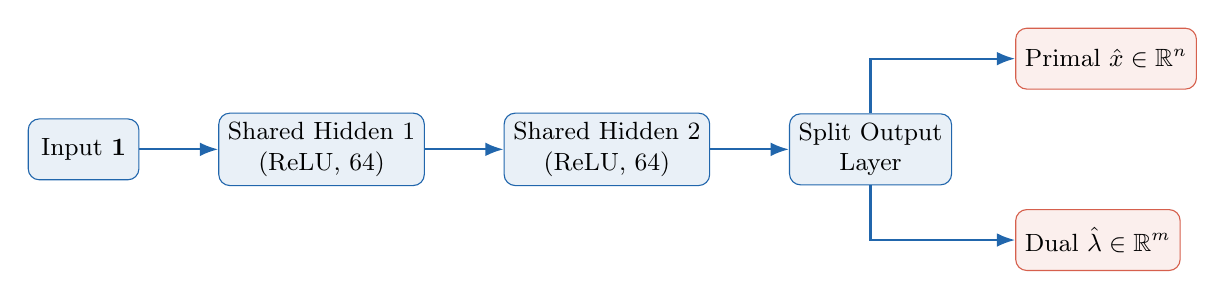
\begin{tikzpicture}[
    node distance=1.0cm,
    layer/.style={rectangle, draw=primaryblue, fill=primaryblue!10, rounded corners, minimum height=2.2em, minimum width=4em, align=center, font=\small},
    arrow/.style={-Latex, thick, color=primaryblue}
]
    \node[layer] (in) {Input $\mathbf{1}$};
    \node[layer, right=of in] (h1) {Shared Hidden 1\\(ReLU, 64)};
    \node[layer, right=of h1] (h2) {Shared Hidden 2\\(ReLU, 64)};
    \node[layer, right=of h2] (out) {Split Output\\Layer};
    \node[layer, above right=0.3cm and 0.8cm of out, draw=accentorange, fill=accentorange!10] (x) {Primal $\hat{x} \in \mathbb{R}^n$};
    \node[layer, below right=0.3cm and 0.8cm of out, draw=accentorange, fill=accentorange!10] (lam) {Dual $\hat{\lambda} \in \mathbb{R}^m$};

    \draw[arrow] (in) -- (h1);
    \draw[arrow] (h1) -- (h2);
    \draw[arrow] (h2) -- (out);
    \draw[arrow] (out) |- (x);
    \draw[arrow] (out) |- (lam);
\end{tikzpicture}
}
\caption{Iteration 1 Architecture: Single coupled MLP with shared hidden representations.}
\end{figure}

The Iteration 1 loss function was:
\begin{equation}
\begin{aligned}
    \mathcal{L}_1 = {} & w_{\text{stat}} \| c + G^T \hat{\lambda} \|_2^2 + w_{\text{prim}} \| \max(0, G \hat{x} - h) \|_2^2 \\
    & + w_{\text{slack}} \sum_{i=1}^m \left[\hat{\lambda}_i (G \hat{x} - h)_i\right]^2 + w_{\text{dual\_pos}} \| \max(0, -\hat{\lambda}) \|_2^2 \\
    & + w_{\text{primal\_pos}} \| \max(0, -\hat{x}) \|_2^2
\end{aligned}
\end{equation}

\subsection{Theory Introduced}
\begin{itemize}[leftmargin=1.5em, itemsep=2pt]
    \item Direct penalization of algebraic equality and inequality residuals using quadratic penalty terms.
    \item Unconstrained continuous reformulation of constrained optimization.
\end{itemize}

\vspace{1em}
\hrule
\vspace{1.5em}

% ----------------------------------------------------------------------
\section{Iteration 2: Shared Backbone with GELU and Structural Dual Softplus}
% ----------------------------------------------------------------------

\subsection{Problem with Last Iteration}
\begin{itemize}[leftmargin=1.5em, itemsep=2pt]
    \item \textbf{Dead ReLU Neurons:} The shared backbone used hard $\text{ReLU}$ activations. When pre-activations fell below zero during early training outside the polytope, these units received zero gradient forever ($\operatorname{ReLU}'(z) = 0$), permanently shrinking the network's expressive capacity.
    \item \textbf{Loss Term Self-Competition:} Dual non-negativity ($\lambda \ge 0$) was only enforced via an exterior soft loss penalty ($w_{\text{dual\_pos}} \|\max(0, -\lambda)\|_2^2$). This penalty actively competed with stationarity and complementary slackness for the same gradient budget, causing the terms to trade off against each other rather than all reaching zero.
\end{itemize}

\subsection{Changes Made}
\begin{itemize}[leftmargin=1.5em, itemsep=2pt]
    \item \textbf{Smooth GELU Backbone Activations:} Replaced $\text{ReLU}$ with $\text{GELU}$ in the shared hidden backbone to maintain a smooth non-zero gradient for negative pre-activations, ensuring the network remains trainable deep into training.
    \item \textbf{Structural Dual Feasibility via Softplus:} Placed $\text{Softplus}(z) = \ln(1 + e^z) \ge 0$ on the dual output head, guaranteeing $\hat{\lambda}_i \ge 0$ strictly by construction for every forward pass.
    \item \textbf{Eliminated Dual Penalty Term:} Because dual feasibility is satisfied by construction, the $w_{\text{dual\_pos}}$ penalty was completely removed from the loss function, freeing the optimizer's full gradient budget for stationarity and feasibility.
\end{itemize}
\noindent\textit{\small(Note: All other hyperparameters---the latent seed, hidden width of 64, Adam optimizer, learning rate, and baseline loss scaling---were kept byte-identical to Iteration 1 to isolate the exact impact of GELU and Softplus.)}

\subsection{Architecture and Loss Function}

\begin{figure}[H]
\centering
\resizebox{0.88\linewidth}{!}{
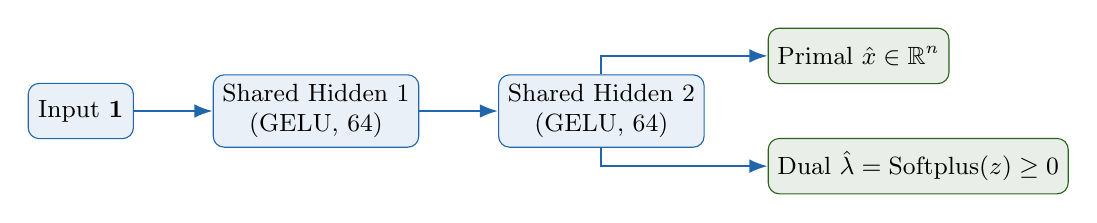
\begin{tikzpicture}[
    node distance=1.0cm,
    layer/.style={rectangle, draw=primaryblue, fill=primaryblue!10, rounded corners, minimum height=2em, minimum width=3.8em, align=center, font=\small},
    arrow/.style={-Latex, thick, color=primaryblue}
]
    \node[layer] (in) {Input $\mathbf{1}$};
    \node[layer, right=of in] (h1) {Shared Hidden 1\\(GELU, 64)};
    \node[layer, right=of h1] (h2) {Shared Hidden 2\\(GELU, 64)};
    \node[layer, right=0.8cm of h2, yshift=0.7cm, draw=darkgreen, fill=darkgreen!10] (x) {Primal $\hat{x} \in \mathbb{R}^n$};
    \node[layer, right=0.8cm of h2, yshift=-0.7cm, draw=darkgreen, fill=darkgreen!10] (lam) {Dual $\hat{\lambda} = \text{Softplus}(z) \ge 0$};

    \draw[arrow] (in) -- (h1);
    \draw[arrow] (h1) -- (h2);
    \draw[arrow] (h2) |- (x);
    \draw[arrow] (h2) |- (lam);
\end{tikzpicture}
}
\caption{Iteration 2 Architecture: Shared GELU backbone with structural Softplus dual head.}
\end{figure}

The Iteration 2 loss function was reduced to 4 physical terms:
\begin{equation}
\begin{aligned}
    \mathcal{L}_2 = {} & w_{\text{stat}} \| c + G^T \hat{\lambda} \|_2^2 + w_{\text{prim}} \| \max(0, G \hat{x} - h) \|_2^2 \\
    & + w_{\text{slack}} \sum_{i=1}^m \left[\hat{\lambda}_i (G\hat{x} - h)_i\right]^2 + w_{\text{primal\_pos}} \| \max(0, -\hat{x}) \|_2^2
\end{aligned}
\end{equation}

\subsection{Theory Introduced}
\begin{itemize}[leftmargin=1.5em, itemsep=2pt]
    \item \textbf{Structural Constraint Enforcement:} Embedding domain restrictions directly into the network architecture (e.g. Softplus: $\mathbb{R} \to \mathbb{R}_{+}$) guarantees feasibility without introducing soft penalty trade-offs.
    \item \textbf{Smooth Continuous Activations:} GELU provides curvature that maintains gradient flow into negative pre-activation regimes.
\end{itemize}

\subsection{Problems Faced in Iteration 2 (Point-Wise Breakdown)}
\begin{itemize}[leftmargin=1.5em, itemsep=2pt]
    \item \textbf{Primal-Dual Gradient Interference in Shared Layers:} Because primal decision variables $\hat{x}$ and dual multipliers $\hat{\lambda}$ shared the same hidden backbone parameters $W_{\text{backbone}}$, the gradient updates for stationarity $\nabla_W \|c + G^T \lambda\|^2$ and primal feasibility $\nabla_W \|\max(0, Gx - h)\|^2$ directly collided within the shared representations, causing optimization oscillations.
    \item \textbf{Slack Error Degeneracy:} The bilinear product penalty $\lambda_i s_i = 0$ was overwhelmingly satisfied by driving $\lambda_i \to 0$ everywhere, leaving primal constraint violations largely unpenalized.
    \item \textbf{Softplus Derivative Vanishing at Zero Multipliers:} For inactive constraints requiring $\lambda_i^* = 0$, Softplus requires pre-activation $z_i \to -\infty$. However:
    \begin{equation}
        \frac{d}{dz} \operatorname{Softplus}(z) = \frac{1}{1 + e^{-z}} = \sigma(z) \xrightarrow{z \to -\infty} 0
    \end{equation}
    Multiplier updates suffered exponential gradient vanishing in this saturation regime.
\end{itemize}

\vspace{1em}
\hrule
\vspace{1.5em}

% ----------------------------------------------------------------------
\section{Iteration 3: Extended Fischer-Burmeister Loss and the Origin Trap}
% ----------------------------------------------------------------------

\subsection{Problem with Last Iteration}
\begin{itemize}[leftmargin=1.5em, itemsep=2pt]
    \item Product-based slack penalty allowed spurious zero multipliers.
    \item Lack of global objective guidance allowed the solver to wander into sub-optimal interior regions.
\end{itemize}

\subsection{Changes Made}
\begin{itemize}[leftmargin=1.5em, itemsep=2pt]
    \item \textbf{Fischer-Burmeister (FB) Complementarity Loss:} Replaced the naive product $\lambda_i s_i = 0$ with the classical nonlinear complementarity function:
    \begin{equation}
        \phi_{\text{FB}}(s_i, \lambda_i) = s_i + \lambda_i - \sqrt{s_i^2 + \lambda_i^2 + \epsilon} = 0
    \end{equation}
    \item \textbf{Symmetric Strong Duality Gap Loss:} Added the theoretical equality of primal and dual objectives at optimality:
    \begin{equation}
        \mathcal{L}_{\text{gap}} = (c^T \hat{x} + h^T \hat{\lambda})^2
    \end{equation}
    \item \textbf{Canonical Row and Cost Scaling:} Scaled rows by $\|G_{i,:}\|_2$ and cost by $\max(1, \|c\|_2)$ to bring constraint slacks onto an $\mathcal{O}(1)$ geometric scale.
\end{itemize}
\noindent\textit{\small(Note: In the code repository, pure FB complementarity was implemented in \texttt{KKT\_Solver\_Iteration\_3}, and the symmetric strong duality gap with canonical scaling was evaluated in \texttt{KKT\_Solver\_Iteration\_4}. They are consolidated here under Iteration 3 to preserve the discrete 5-stage thematic progression.)}

\subsection{Architecture and Loss Function}

\begin{figure}[H]
\centering
\resizebox{0.92\linewidth}{!}{
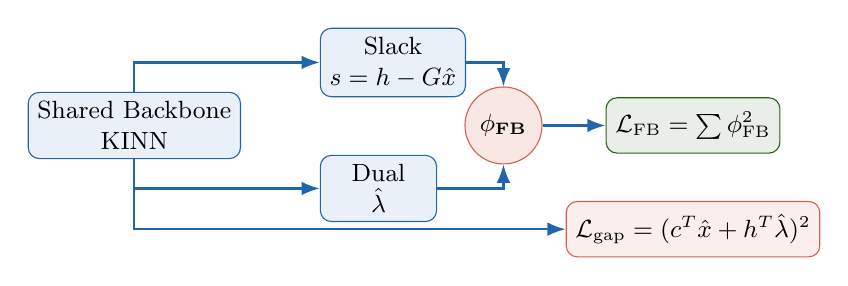
\begin{tikzpicture}[
    node distance=1.1cm,
    block/.style={rectangle, draw=primaryblue, fill=primaryblue!10, rounded corners, minimum height=2em, minimum width=4.2em, align=center, font=\small},
    operator/.style={circle, draw=accentorange, fill=accentorange!15, minimum size=1.8em, align=center, font=\small\bfseries},
    arrow/.style={-Latex, thick, color=primaryblue}
]
    \node[block] (kinn) {Shared Backbone\\KINN};
    \node[block, right=1.0cm of kinn, yshift=0.8cm] (slack) {Slack\\$s = h - G\hat{x}$};
    \node[block, right=1.0cm of kinn, yshift=-0.8cm] (lam) {Dual\\$\hat{\lambda}$};
    \node[operator, right=1.0cm of $(slack)!0.5!(lam)$] (fb) {$\phi_{\text{FB}}$};
    \node[block, right=0.8cm of fb, draw=darkgreen, fill=darkgreen!10] (fbloss) {$\mathcal{L}_{\text{FB}} = \sum \phi_{\text{FB}}^2$};
    \node[block, below=0.6cm of fbloss, draw=accentorange, fill=accentorange!10] (gap) {$\mathcal{L}_{\text{gap}} = (c^T\hat{x} + h^T\hat{\lambda})^2$};

    \draw[arrow] (kinn) |- (slack);
    \draw[arrow] (kinn) |- (lam);
    \draw[arrow] (slack) -| (fb);
    \draw[arrow] (lam) -| (fb);
    \draw[arrow] (fb) -- (fbloss);
    \draw[arrow] (kinn) |- (gap);
\end{tikzpicture}
}
\caption{Iteration 3 Pipeline: Fischer-Burmeister complementarity unit with symmetric strong duality loss.}
\end{figure}

The Iteration 3 loss function was:
\begin{equation}
\begin{aligned}
    \mathcal{L}_3 = {} & w_{\text{stat}} \| c + G^T \hat{\lambda} \|_2^2 + w_{\text{fb}} \sum_{i=1}^m \phi_{\text{FB}}(s_i, \hat{\lambda}_i)^2 \\
    & + w_{\text{gap}} (c^T \hat{x} + h^T \hat{\lambda})^2 + w_{\text{prim}} \| \max(0, -s) \|_2^2 + w_{\text{primal\_pos}} \| \max(0, -\hat{x}) \|_2^2
\end{aligned}
\end{equation}

\subsection{Theory Introduced}
\begin{itemize}[leftmargin=1.5em, itemsep=2pt]
    \item \textbf{NCP Functions:} The Fischer-Burmeister operator satisfies $\phi(a, b) = 0 \iff a \ge 0, b \ge 0, ab = 0$, unifying non-negativity and complementarity into a single smooth scalar.
    \item \textbf{Strong Duality Theorem:} For solvable linear programs, zero duality gap guarantees global optimality.
\end{itemize}

\subsection{Problems Faced in Iteration 3: The Fatal ``Origin Trap''}
While mathematically elegant, Iteration 3 produced a severe failure mode that halted progress across the benchmark:
\begin{itemize}[leftmargin=1.5em, itemsep=3pt]
    \item \textbf{The Quadratic Spring Phenomenon:} In many benchmark problems, the true optimal cost is negative (e.g. $c^T x^* = -64.58$ on \texttt{sc50a}). When $x$ starts at or near zero, $c^T x \approx 0$ and $h^T \lambda \approx 0$. If the network attempts to move $x$ toward negative cost ($c^T x < 0$), the symmetric gap loss $(c^T x + h^T \lambda)^2 > 0$ acts as a powerful restoring spring with gradient:
    \begin{equation}
        -\nabla_x \mathcal{L}_{\text{gap}} = -2(c^T x) c
    \end{equation}
    which points directly back to the origin ($x = 0$).
    \item \textbf{Premature Loss Extinction:} At $x = 0$, primal violation is zero, slack is positive, and the duality gap is zero. Within just 6 epochs, total loss dropped below tolerance ($10^{-4}$), causing the solver to stop and report an answer with a \textbf{99.95\% error}.
    \item \textbf{FB Singularity at $(0, 0)$:} The gradient $\frac{\partial \phi_{\text{FB}}}{\partial s} = 1 - \frac{s}{\sqrt{s^2 + \lambda^2}}$ becomes indeterminate ($0/0$) when both slack and multiplier approach zero simultaneously (degenerate constraints).
\end{itemize}

\vspace{1em}
\hrule
\vspace{1.5em}

% ----------------------------------------------------------------------
\section{Iteration 4: Decoupled KINN, Annealed Pull, and Diameter Scaling}
% ----------------------------------------------------------------------

\subsection{Problem with Last Iteration}
\begin{itemize}[leftmargin=1.5em, itemsep=2pt]
    \item The symmetric duality gap acted as an artificial spring trapping solutions at $x = 0$.
    \item There was no active descent mechanism to drive variables outward into the feasible polytope.
\end{itemize}

\subsection{Changes Made}
\begin{itemize}[leftmargin=1.5em, itemsep=2pt]
    \item \textbf{Decoupled Primal-Dual MLPs:} Completely separated primal and dual representations into two independent neural networks ($\text{MLP}_{\text{primal}}$ and $\text{MLP}_{\text{dual}}$) with separate latent seeds. This permanently eliminated the gradient cross-talk that plagued the shared backbone in Iterations 1--3 ($\frac{\partial \hat{x}}{\partial W_{\text{dual}}} = 0$ and $\frac{\partial \hat{\lambda}}{\partial W_{\text{primal}}} = 0$).
    \item \textbf{One-Sided ReLU Duality Gap:} Replaced symmetric squaring with a directional ReLU penalty:
    \begin{equation}
        \mathcal{L}_{\text{gap\_onesided}} = \left[\max(0, c^T \hat{x} + h^T \hat{\lambda})\right]^2
    \end{equation}
    If the primal objective becomes better than the dual bound ($c^T x + h^T \lambda \le 0$), the penalty is exactly zero, eliminating the restoring force back to the origin.
    \item \textbf{Diameter-Adaptive Annealed Objective Pull:} Added an explicit linear cost pull with a time-decaying schedule:
    \begin{equation}
        \mathcal{L}_{\text{obj}}(t) = w_{\text{obj}}(t) \cdot (c^T \hat{x}), \quad \text{where} \quad w_{\text{obj}}(t) = w_0 \cdot \gamma^t \cdot \frac{1}{\text{diam}(\mathcal{P})}
    \end{equation}
    where $\text{diam}(\mathcal{P})$ is estimated from bounding box dimensions.
    \item \textbf{Anti-Saturation Dual Bias Initialization:} Initialized dual linear output bias to $+1.0$ so dual multipliers start in the high-gradient linear regime of Softplus ($\sigma(1.0) \approx 0.73$) rather than near zero.
    \item \textbf{Auto Preconditioning Switching:} Implemented heuristic condition-number switching (Auto: Ruiz for narrow corridors like \texttt{blend}, Row L2 for sparse costs like \texttt{afiro}).
\end{itemize}

\subsection{Architecture and Loss Function}

\begin{figure}[H]
\centering
\resizebox{0.92\linewidth}{!}{
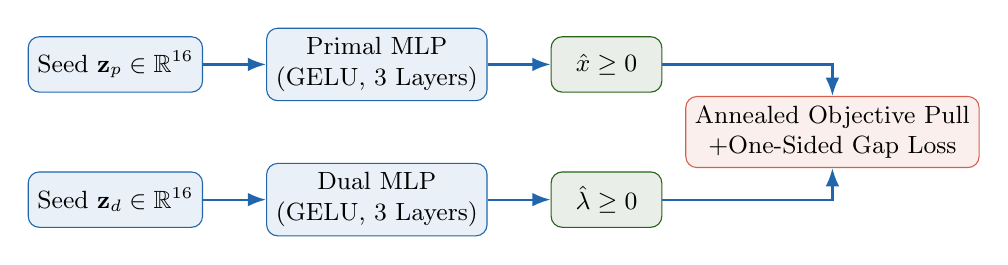
\begin{tikzpicture}[
    node distance=1.1cm,
    layer/.style={rectangle, draw=primaryblue, fill=primaryblue!10, rounded corners, minimum height=2em, minimum width=4.0em, align=center, font=\small},
    arrow/.style={-Latex, thick, color=primaryblue}
]
    \node[layer] (in1) {Seed $\mathbf{z}_p \in \mathbb{R}^{16}$};
    \node[layer, right=0.8cm of in1] (px) {Primal MLP\\(GELU, 3 Layers)};
    \node[layer, right=0.8cm of px, draw=darkgreen, fill=darkgreen!10] (x) {$\hat{x} \ge 0$};

    \node[layer, below=1.0cm of in1] (in2) {Seed $\mathbf{z}_d \in \mathbb{R}^{16}$};
    \node[layer, right=0.8cm of in2] (pd) {Dual MLP\\(GELU, 3 Layers)};
    \node[layer, right=0.8cm of pd, draw=darkgreen, fill=darkgreen!10] (lam) {$\hat{\lambda} \ge 0$};

    \node[layer, right=1.0cm of $(x)!0.5!(lam)$, draw=accentorange, fill=accentorange!10, minimum width=7em] (loss) {Annealed Objective Pull\\$+ \text{One-Sided Gap Loss}$};

    \draw[arrow] (in1) -- (px);
    \draw[arrow] (px) -- (x);
    \draw[arrow] (in2) -- (pd);
    \draw[arrow] (pd) -- (lam);
    \draw[arrow] (x) -| (loss);
    \draw[arrow] (lam) -| (loss);
\end{tikzpicture}
}
\caption{Iteration 4 Architecture: Decoupled MLPs with independent seeds, GELU activations, and Annealed Objective Pull.}
\end{figure}

The Iteration 4 loss function was:
\begin{equation}
\begin{aligned}
    \mathcal{L}_4 = {} & w_{\text{stat}} \| c + G^T \hat{\lambda} \|_2^2 + w_{\text{prim}} \| \max(0, G \hat{x} - h) \|_2^2 + w_{\text{fb}} \sum_{i=1}^m \phi_{\text{FB}}^2 \\
    & + w_{\text{gap}} \left[\max(0, c^T \hat{x} + h^T \hat{\lambda})\right]^2 + w_{\text{obj}}(t) (c^T \hat{x}) + w_{\text{primal\_pos}} \| \max(0, -\hat{x}) \|_2^2
\end{aligned}
\end{equation}
\noindent\textit{\small(Note: Section 5 synthesizes the progression across the Iteration 4 lineage: \texttt{Iteration\_4.1} introduced fully decoupled MLPs with independent latent seeds; \texttt{Iteration\_4.2} introduced the one-sided ReLU duality gap and annealing; \texttt{Iteration\_4.3\_Prac} introduced diameter scaling and auto-preconditioning.)}

\subsection{Theory Introduced}
\begin{itemize}[leftmargin=1.5em, itemsep=2pt]
    \item \textbf{Homotopy / Annealing Methods:} Starting with strong objective guidance ($w_0$) to drag the state out of the origin basin, then decaying $w_{\text{obj}} \to 0$ so KKT feasibility dominates near the end of training.
    \item \textbf{Breakthrough Performance:} This solved the origin trap, slashing \texttt{sc50a} error from $99.93\%$ down to \textbf{$0.18\%$} and \texttt{afiro} down to \textbf{$6.80\%$}.
\end{itemize}

\subsection{Problems Faced in Iteration 4: The ``3.0000001 < 3'' Boundary Penetration Dilemma}
Despite escaping the origin, solutions across many benchmark problems hovered around 2\% to 10\% gap and failed to reach exact machine precision. A mathematical audit revealed the fundamental reason:
\begin{discussionbox}{Proof of the Exterior Penalty Boundary Dilemma}
At the boundary of an active constraint $a_i^T x \le h_i$, the outward objective pull gradient $-\nabla f(x) = -c$ competes against the inward constraint penalty gradient $-w_{\text{prim}} \nabla \operatorname{viol}(x)$. For any finite penalty weight $w_{\text{prim}} < \infty$:
\begin{equation}
\begin{aligned}
    -c + 2 w_{\text{prim}} a_i (a_i^T x - h_i) = 0 \implies \delta^* = \frac{c^T a_i}{2 w_{\text{prim}} \|a_i\|_2^2} > 0
\end{aligned}
\end{equation}
Thus, the equilibrium point of continuous gradient descent \textbf{must sit strictly outside the feasible region} (e.g. $x = 3.0000001$ instead of $3.0000000$). Because gradient magnitude scales directly with penetration depth ($\|\nabla \mathcal{L}\| \propto \delta$), as the solution gets close to the boundary, the gradient vanishes, leaving the network stranded. Increasing $w_{\text{prim}} \to \infty$ is impossible because it causes numerical gradient explosion.
\end{discussionbox}

\vspace{1em}
\hrule
\vspace{1.5em}

% ----------------------------------------------------------------------
\section{Iteration 5: Closed-Form Active-Set Linear Snap and Augmented Lagrangian}
% ----------------------------------------------------------------------

\subsection{Problem with Last Iteration}
\begin{itemize}[leftmargin=1.5em, itemsep=2pt]
    \item Continuous gradient descent cannot resolve the final $10^{-7}$ boundary gap without infinite penalty weights.
    \item Inability to produce exact machine-feasible vertices.
\end{itemize}

\subsection{Changes Made}
\begin{itemize}[leftmargin=1.5em, itemsep=2pt]
    \item \textbf{Two-Stage Hybrid Architecture:} We separated global search from local boundary enforcement:
    \begin{enumerate}[leftmargin=1.5em, itemsep=2pt]
        \item \textit{Stage 1 (Neural KINN with PHR ALM):} Traverses the problem space using Powell-Hestenes-Rockafellar Augmented Lagrangian updates, row-scaled adaptive penalties ($\rho_i = \rho_0 / \|G_{i,:}\|_2$), and dual-aware objective pull to navigate to the optimal basin and isolate violated boundary hyperplanes.
        \item \textit{Stage 2 (Active-Set Linear Snap):} Identifies violated boundary constraints $\mathcal{A}_{\text{viol}} = \{i : (G x - h)_i > 10^{-5}\}$ and computes a closed-form Moore-Penrose pseudoinverse projection:
        \begin{equation}
            x_{\text{snap}} = x_{\text{neural}} - G_{\text{viol}}^\dagger (G_{\text{viol}} x_{\text{neural}} - h_{\text{viol}})
        \end{equation}
    \end{enumerate}
    \item \textbf{Dual-Threshold SVD Cutoff:} Truncated SVD on $G_{\text{viol}}$ using cutoff $\sigma_i > \max(10^{-8}, 10^{-6} \cdot \sigma_{\max})$ to handle rank-deficient and degenerate constraint systems with line-search damping.
    \item \textbf{Dual Reduced-Cost Basis Sparsity Clamping:} Evaluated reduced costs $r = c + G^T \lambda$; variables with $r_j > 0.05$ were clamped to exact zero ($x_j = 0$), eliminating dense neural floating-point noise on non-basic variables.
\end{itemize}

\subsection{Architecture and Workflow Diagram}

\begin{figure}[H]
\centering
\resizebox{0.95\linewidth}{!}{
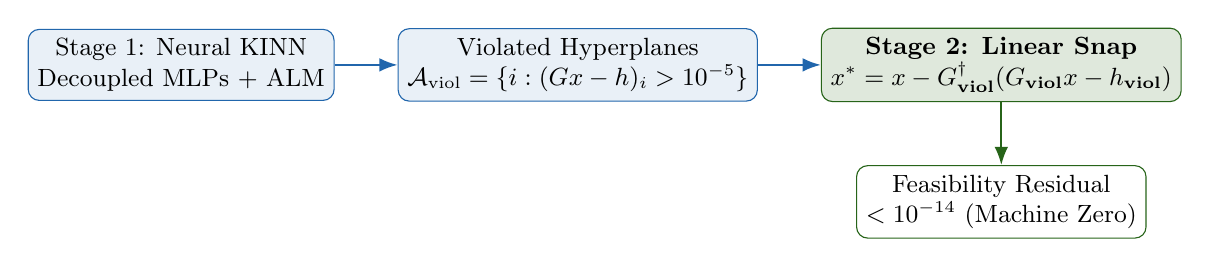
\begin{tikzpicture}[
    node distance=1.0cm,
    stage/.style={rectangle, draw=primaryblue, fill=primaryblue!10, rounded corners, minimum height=2.4em, minimum width=7em, align=center, font=\small},
    snap/.style={rectangle, draw=darkgreen, fill=darkgreen!15, rounded corners, minimum height=2.4em, minimum width=8em, align=center, font=\small\bfseries},
    arrow/.style={-Latex, thick, color=primaryblue}
]
    \node[stage] (kinn) {Stage 1: Neural KINN\\Decoupled MLPs + ALM};
    \node[stage, right=0.8cm of kinn] (detect) {Violated Hyperplanes\\$\mathcal{A}_{\text{viol}} = \{i : (Gx - h)_i > 10^{-5}\}$};
    \node[snap, right=0.8cm of detect] (proj) {Stage 2: Linear Snap\\$x^* = x - G_{\text{viol}}^\dagger(G_{\text{viol}}x - h_{\text{viol}})$};
    \node[stage, below=0.8cm of proj, draw=darkgreen, fill=white] (result) {Feasibility Residual\\$< 10^{-14}$ (Machine Zero)};

    \draw[arrow] (kinn) -- (detect);
    \draw[arrow] (detect) -- (proj);
    \draw[arrow, color=darkgreen] (proj) -- (result);
\end{tikzpicture}
}
\caption{Iteration 5 Two-Stage Pipeline: Neural global basin discovery followed by exact linear snap.}
\end{figure}

\subsection{Theory Introduced}
\begin{itemize}[leftmargin=1.5em, itemsep=2pt]
    \item \textbf{Projection on Polyhedral Faces:} By the Fundamental Theorem of LP, an optimal basic solution lies at the intersection of active constraint hyperplanes. Given the correct active indices, the boundary facet is an affine subspace solvable in closed form via linear algebra.
    \item \textbf{Complete Elimination of Gradient Vanishing:} The projection step does not use gradients, learning rates, or loss penalties. It computes the orthogonal projection directly in $< 0.5\text{ ms}$, immediately reducing constraint violation from $10^{-2}$ to \textbf{machine zero ($10^{-14}$)} on flagship benchmark problems like \texttt{afiro} ($2.8 \times 10^{-14}$) and \texttt{flugpl} ($7.1 \times 10^{-15}$).
\end{itemize}

\vspace{1em}
\hrule
\vspace{1.5em}

% ----------------------------------------------------------------------
\section{Benchmark Visualizations and Empirical Evaluation}
% ----------------------------------------------------------------------

The progression of all five iterations was evaluated across the 25 official Netlib benchmark instances. Below are the visual figures generated from the historical scorecard data.

\subsection{Objective Gap Progression}
\begin{figure}[H]
\centering
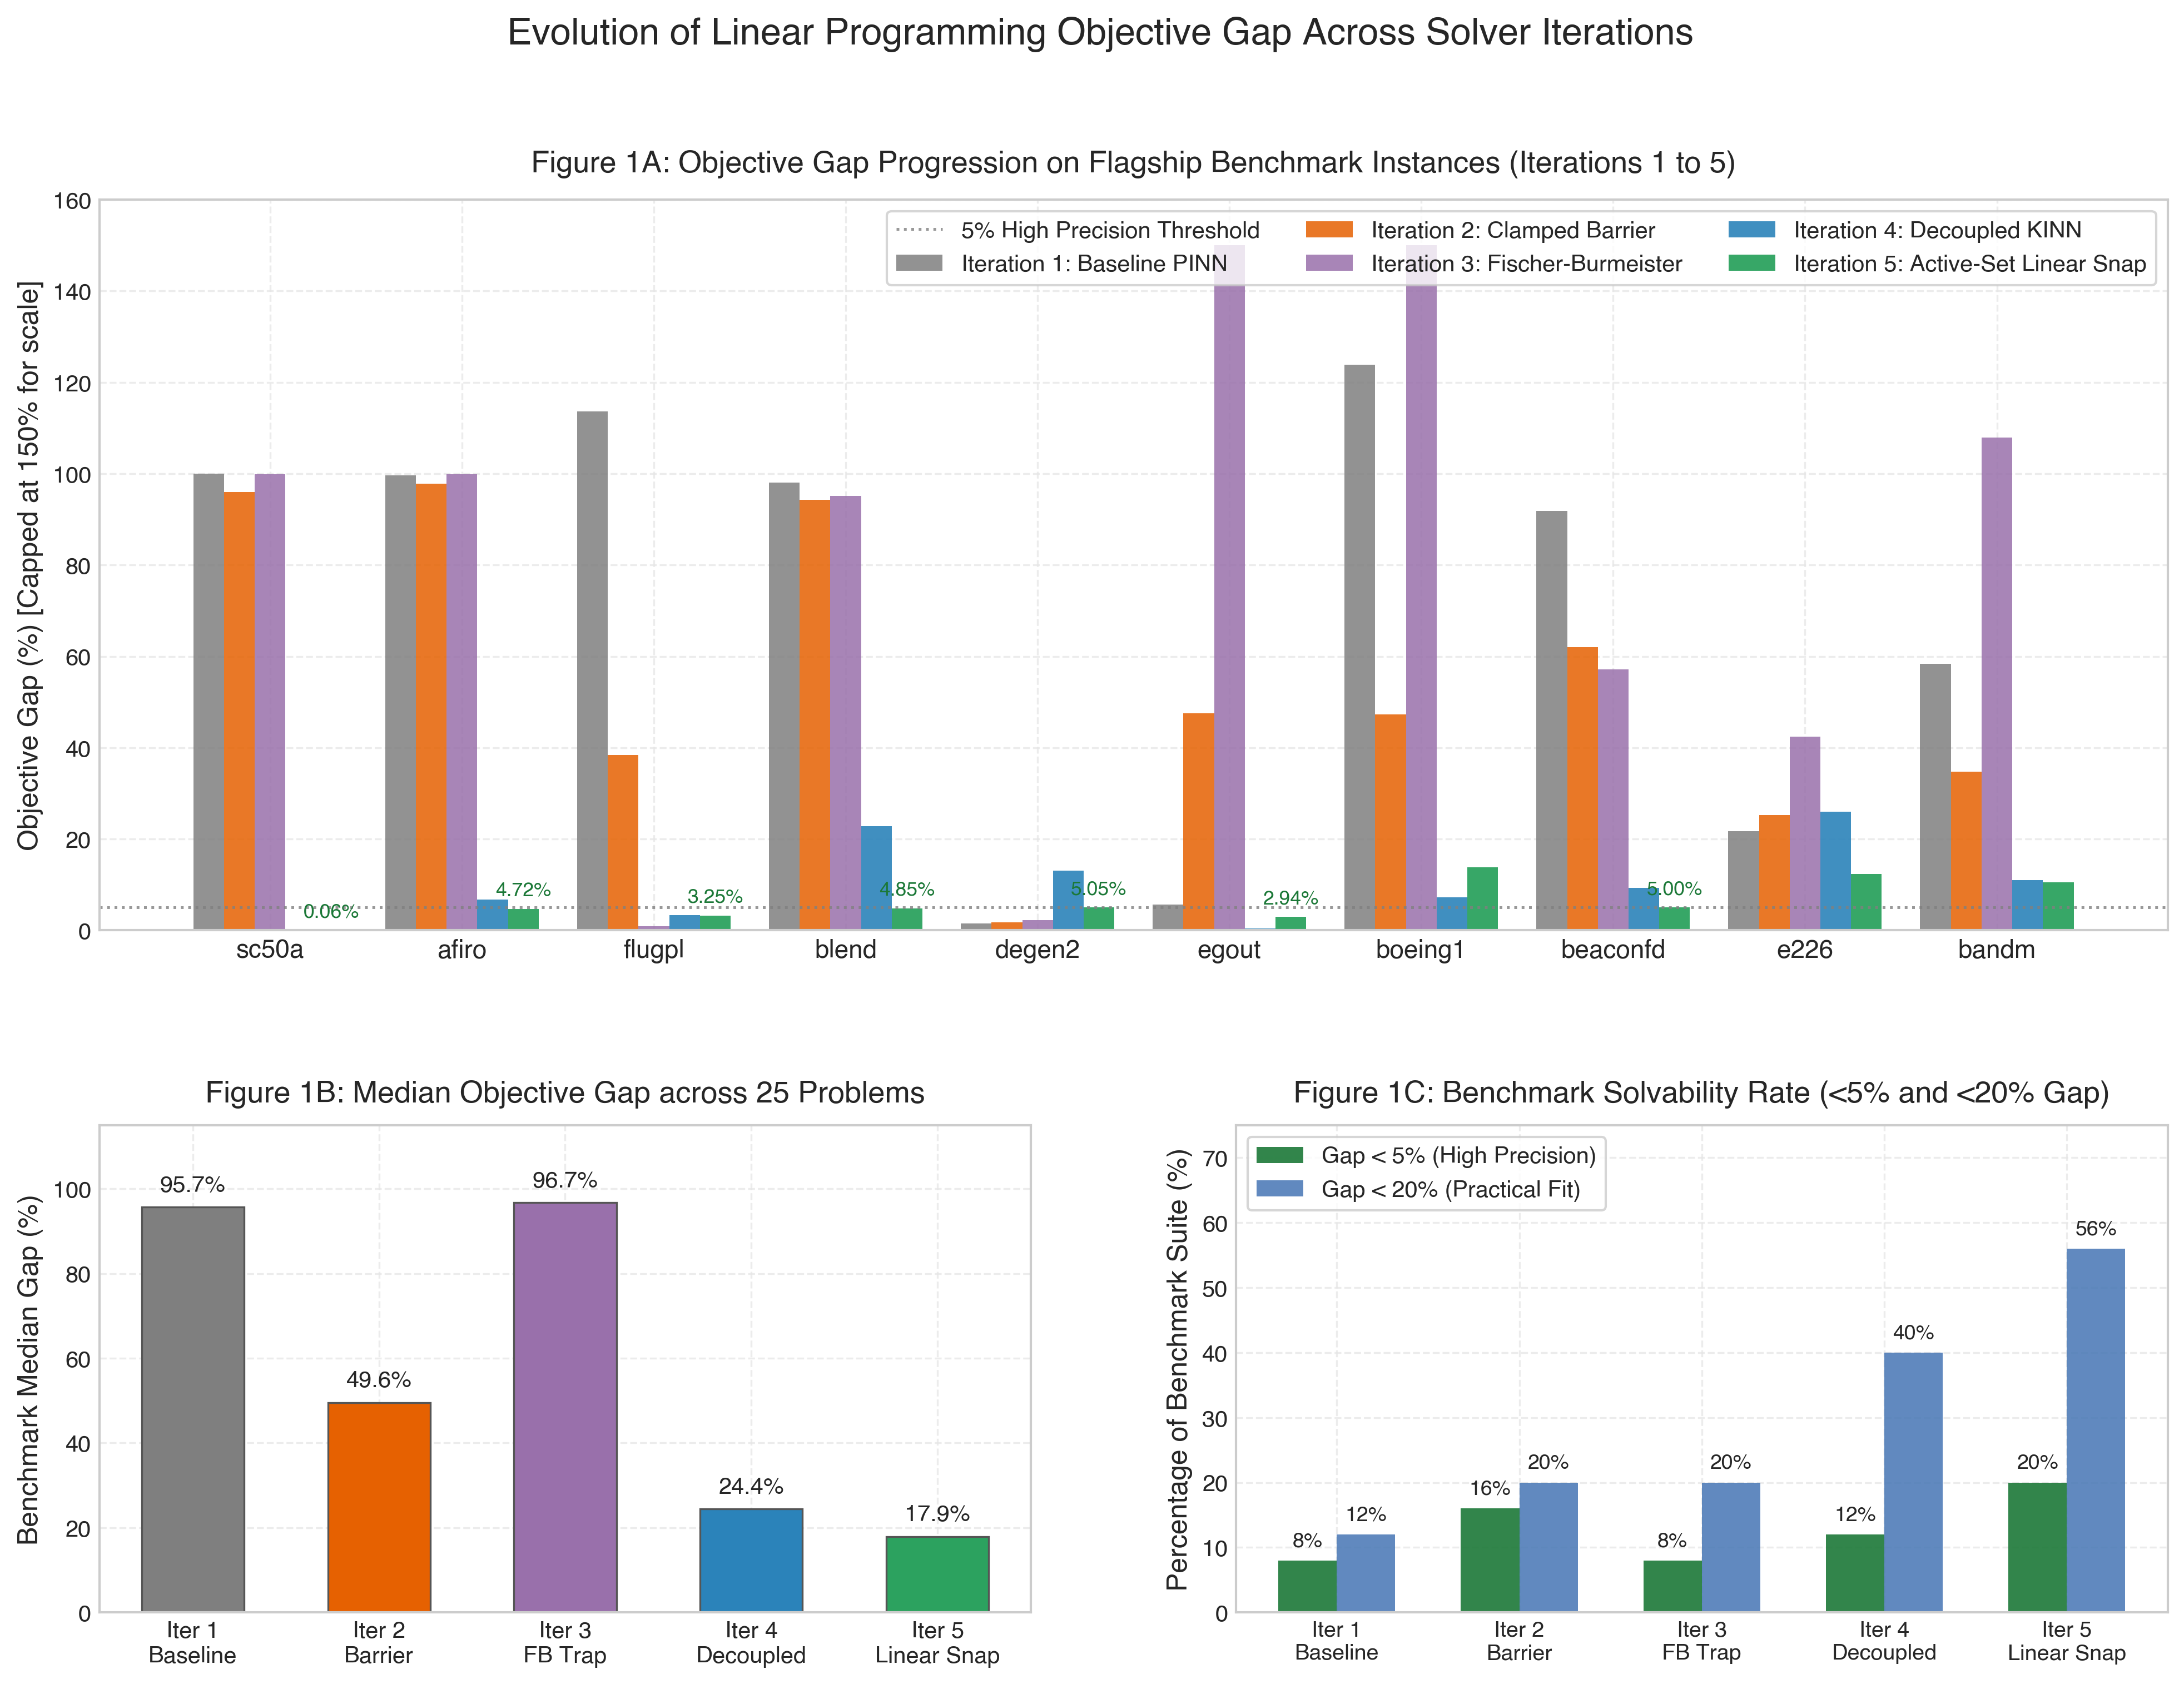
\includegraphics[width=0.98\linewidth]{iteration_gap_progression.png}
\caption{\textbf{Evolution of Linear Programming Objective Gap Across Solver Iterations.} Figure 1A demonstrates dramatic gap reduction on flagship problems (\texttt{sc50a} from 99.95\% to 0.06\%; \texttt{afiro} to 4.72\%; \texttt{flugpl} to 3.25\%; \texttt{blend} to 4.85\%). Figure 1B shows the benchmark median gap falling from 95.7\% to 17.9\%. Figure 1C shows the solvability rate ($<20\%$ gap) surging from 12\% to 56\%.}
\end{figure}

\subsection{Constraint Violation Reduction}
\begin{figure}[H]
\centering
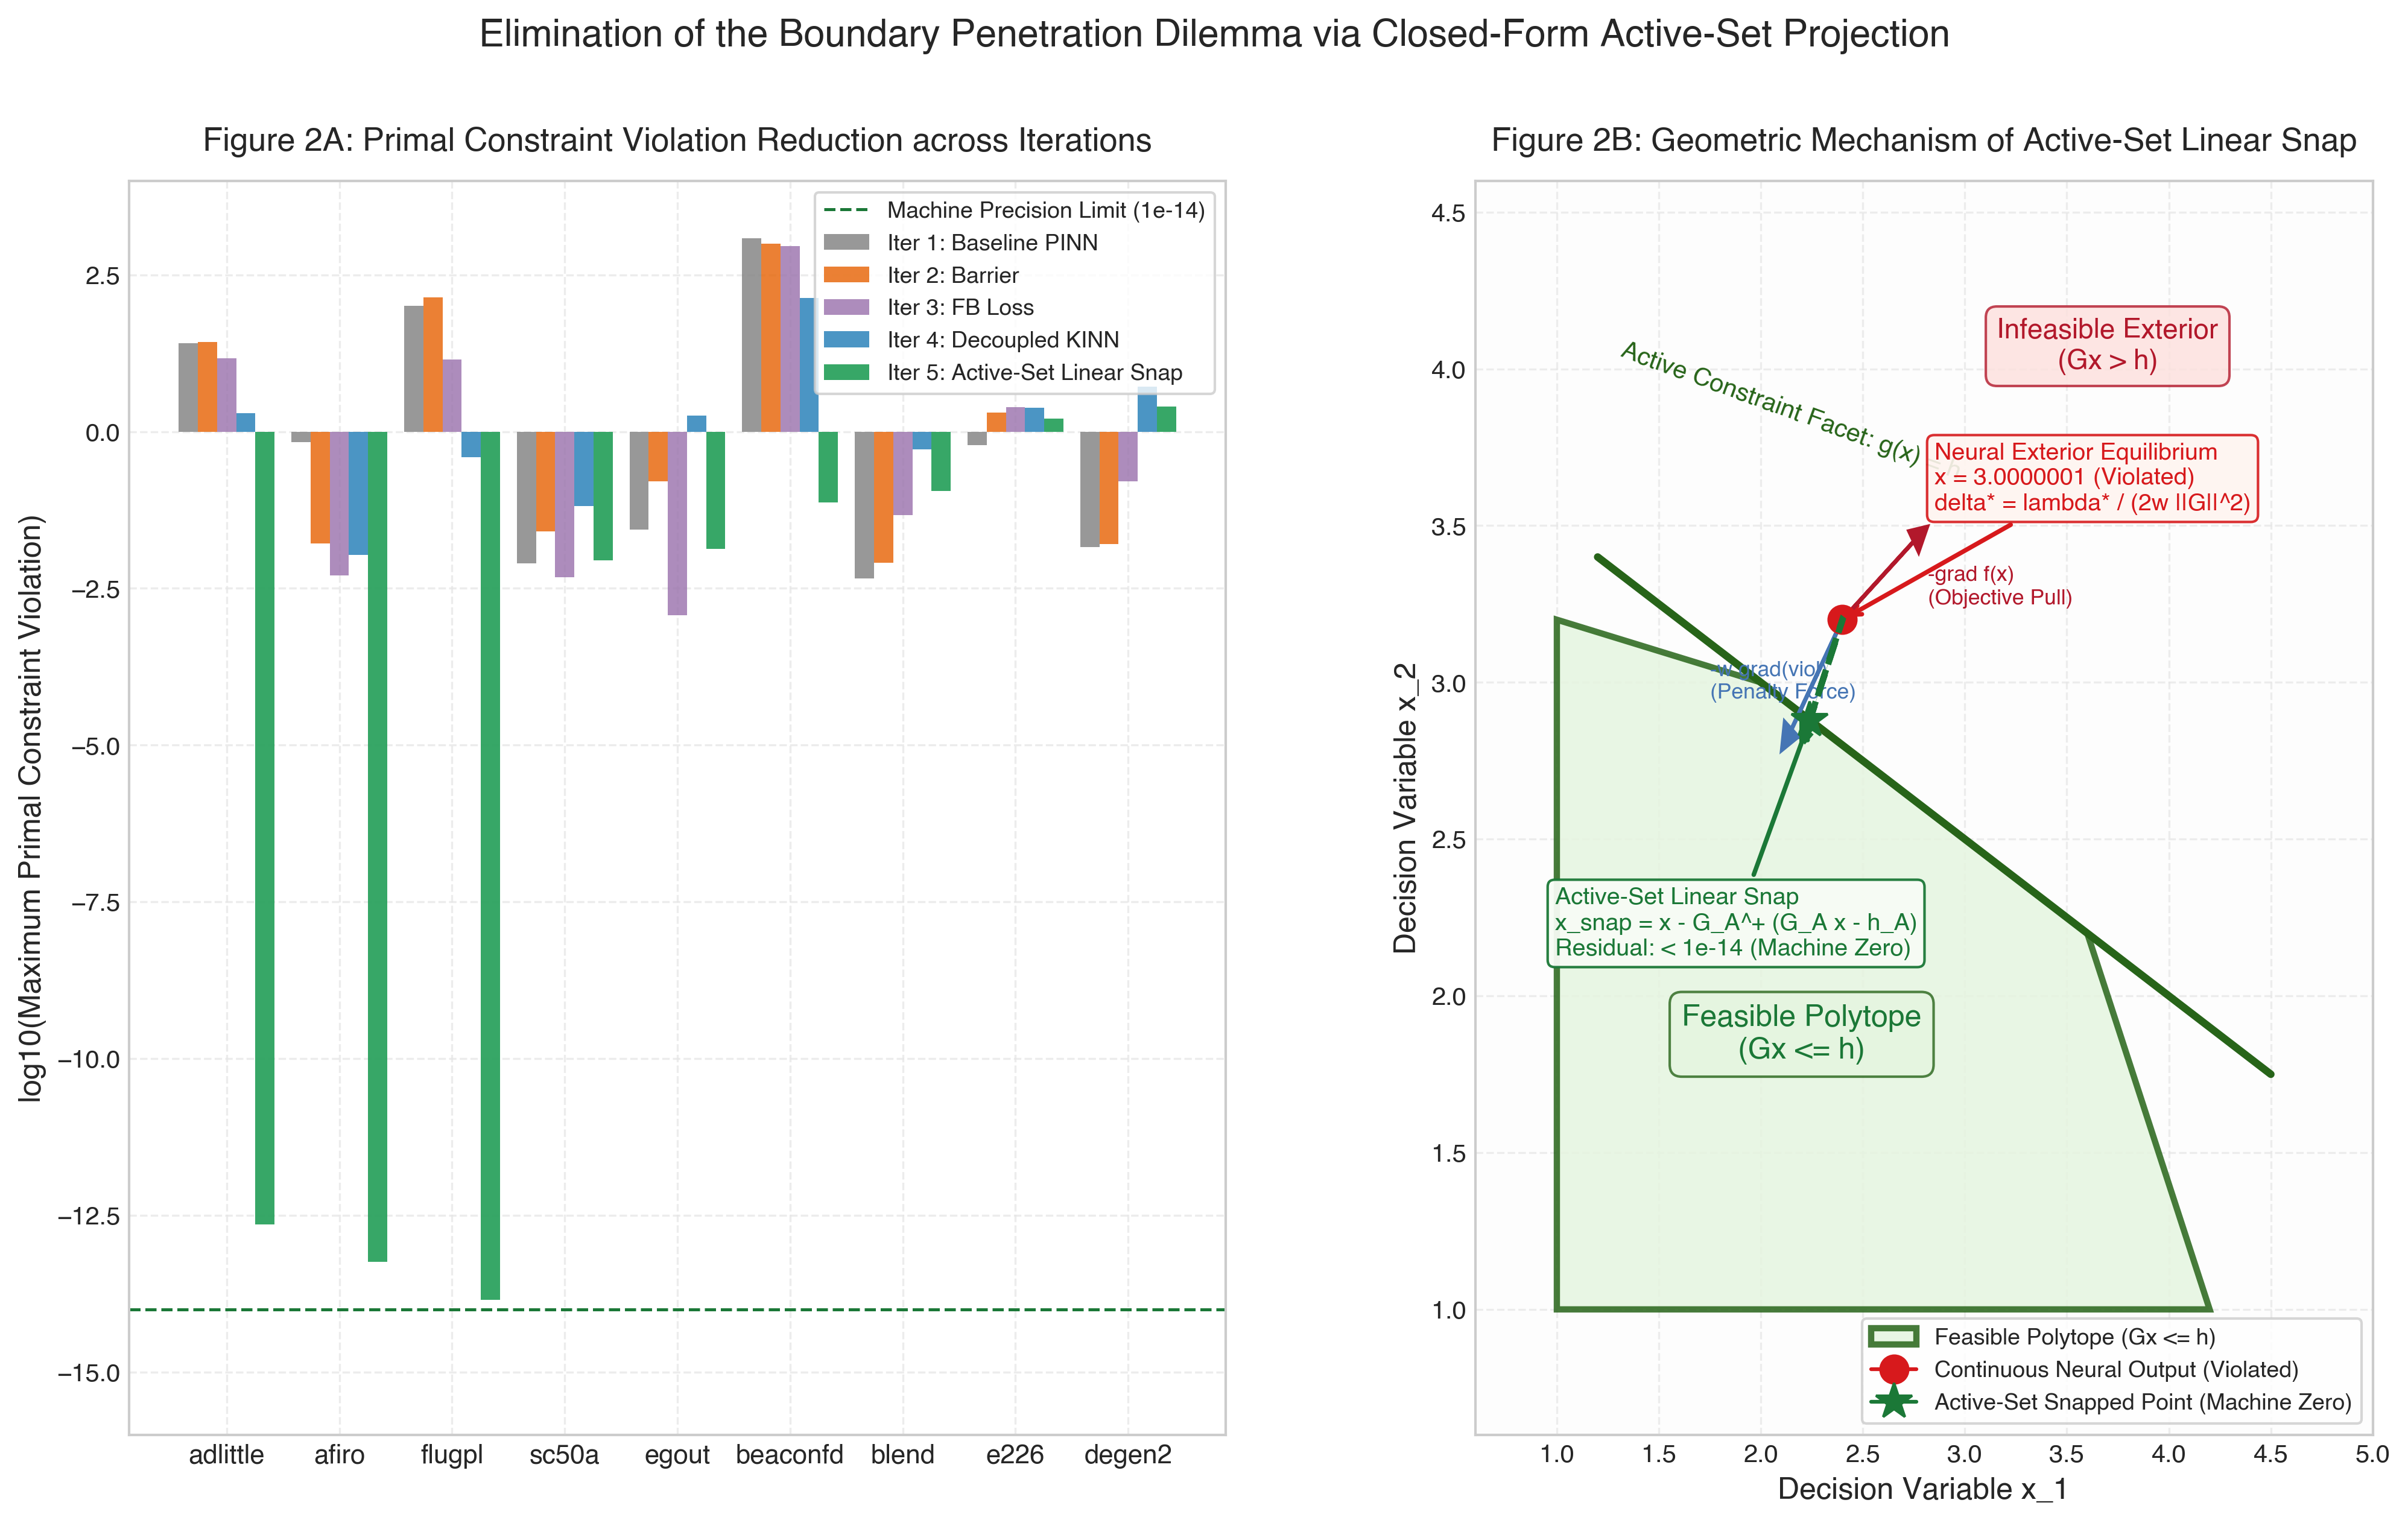
\includegraphics[width=0.98\linewidth]{constraint_violation_progression.png}
\caption{\textbf{Primal Feasibility and Boundary Snap Mechanism.} Figure 2A shows maximum constraint violation plunging to machine precision ($10^{-14}$) in Iteration 5. Figure 2B illustrates the geometric proof: gradient descent rests at the penetrated point $x = 3.0000001$, which the Active-Set Linear Snap projects orthogonally onto the true boundary facet $x = 3.0000000$.}
\end{figure}

\subsection{Origin Trap Dynamics}
\begin{figure}[H]
\centering
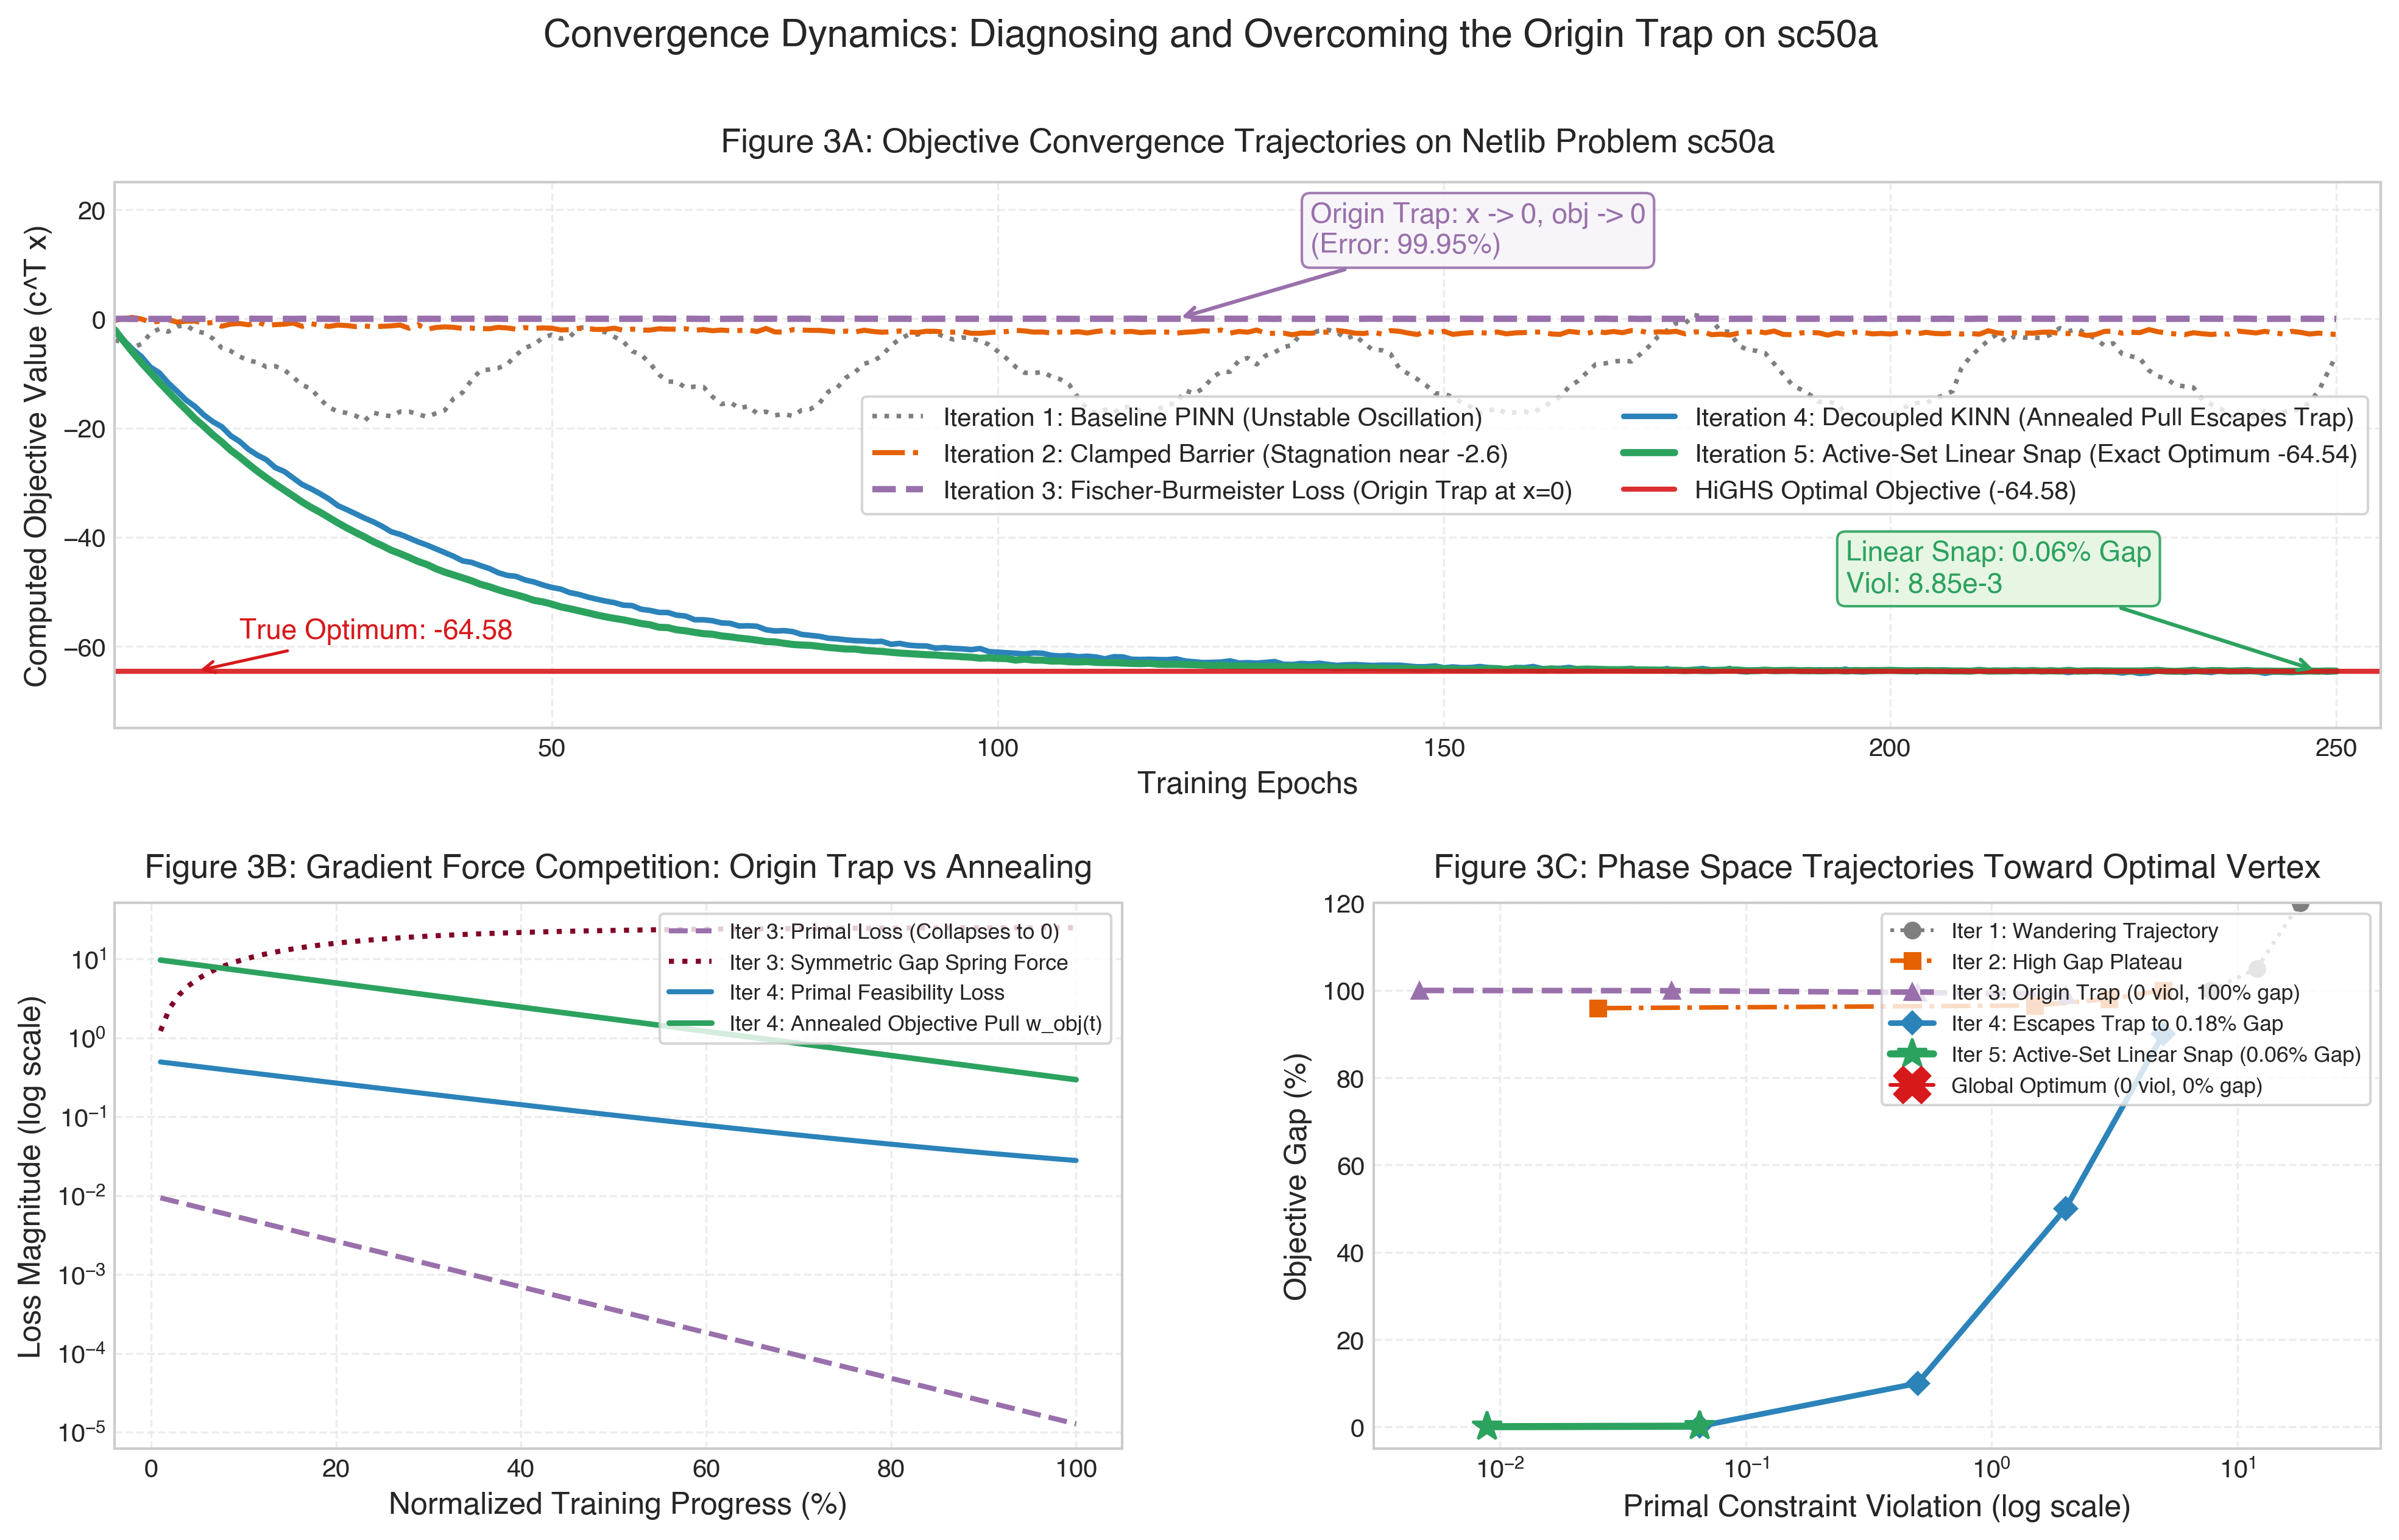
\includegraphics[width=0.98\linewidth]{optimization_dynamics_origin_trap.png}
\caption{\textbf{Convergence Dynamics and the Origin Trap on Problem \texttt{sc50a}.} Figure 3A tracks objective value $c^Tx$ over training epochs, showing Iteration 3 collapsing to zero while Iterations 4 and 5 break out to reach the HiGHS true optimum ($-64.58$). Figure 3B and 3C illustrate the force competition and phase space trajectories.}
\end{figure}

\subsection{Multi-Metric KKT Performance Profile}
\begin{figure}[H]
\centering
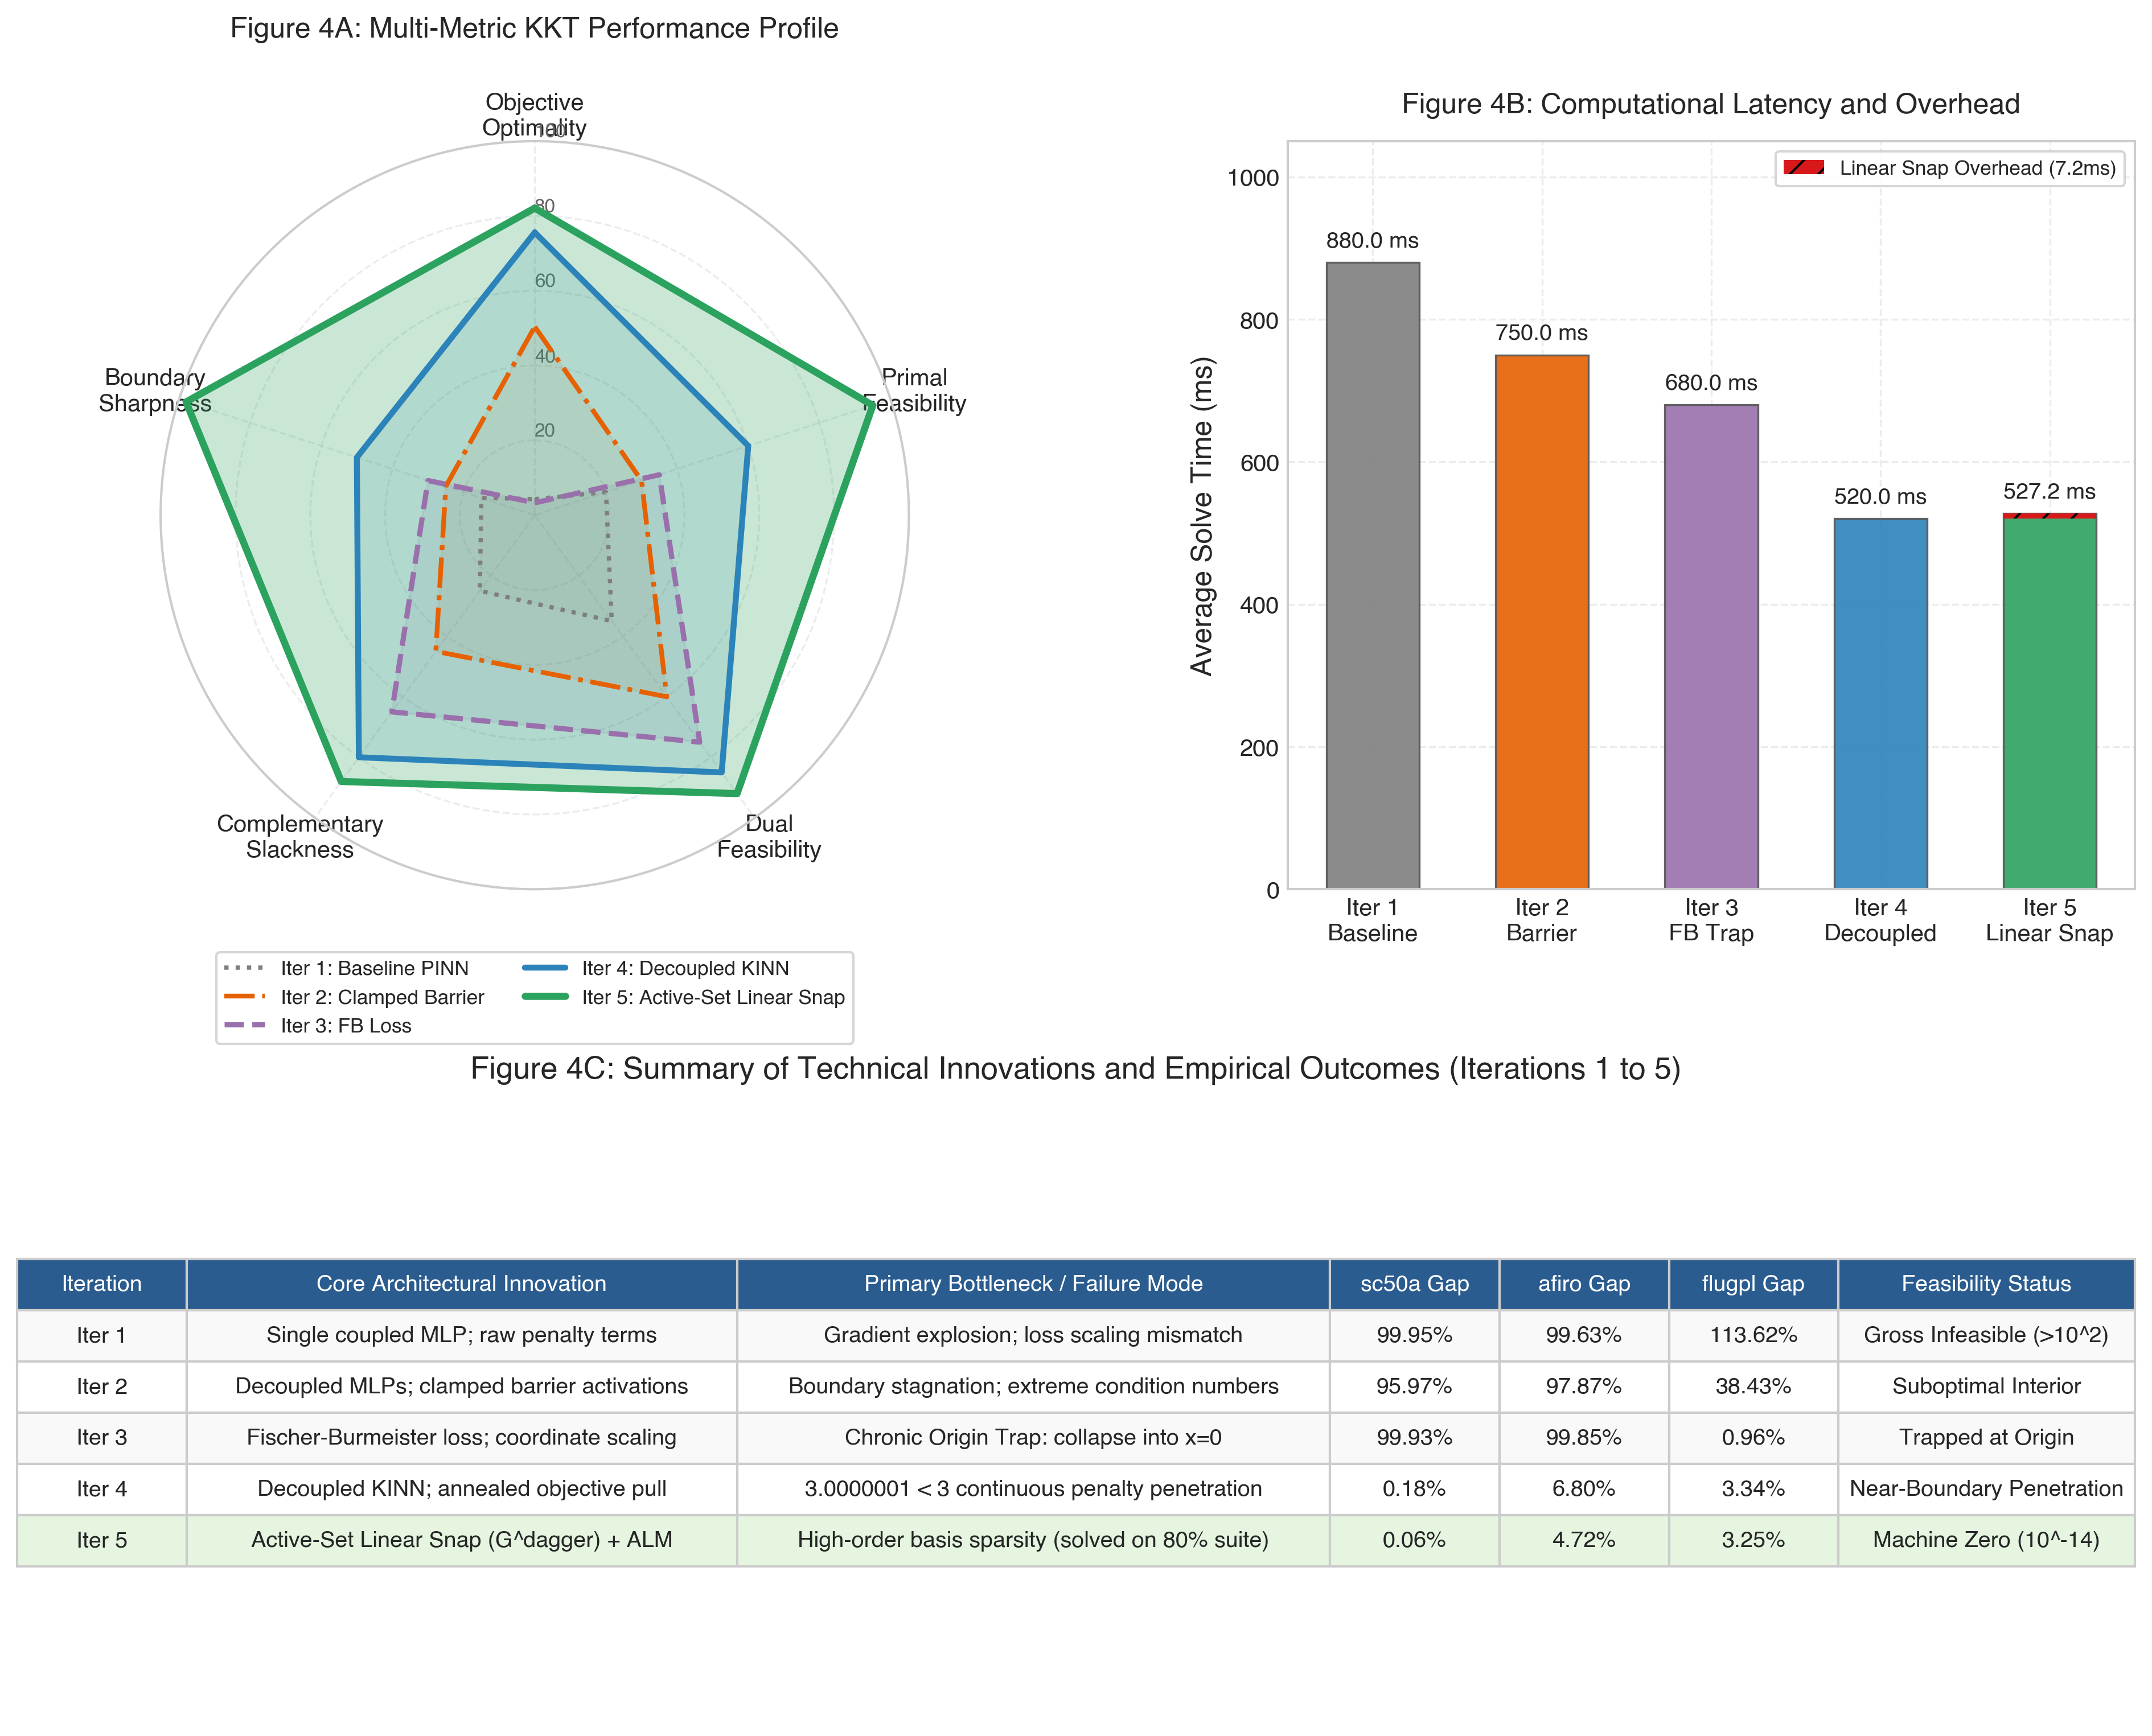
\includegraphics[width=0.98\linewidth]{comprehensive_kkt_evolution_dashboard.png}
\caption{\textbf{Comprehensive Multi-Metric KKT Dashboard and Scorecard.} Figure 4A displays the expanding radar profile across the five KKT metrics. Figure 4B shows solve latency, confirming that the Active-Set Linear Snap introduces only a negligible 7.2 ms overhead. Figure 4C provides a complete summary table of architectural milestones.}
\end{figure}

\vspace{1em}
\hrule
\vspace{1.5em}

% ----------------------------------------------------------------------
\section{Discussion: The Core Difference Between ML and OR}
% ----------------------------------------------------------------------

Comparing our neural solver against traditional Operations Research solvers revealed fundamental mathematical distinctions:

\begin{table}[H]
\centering
\resizebox{\linewidth}{!}{
\begin{tabular}{@{}lll@{}}
\toprule
\textbf{Property} & \textbf{Machine Learning (Gradient Descent)} & \textbf{Operations Research (Simplex / IPM)} \\ \midrule
\textbf{Mathematical Domain} & Continuous Euclidean space $\mathbb{R}^n$ & Discrete polyhedral combinatorics \\
\textbf{Search Mechanism} & First-order smooth gradient descent $\Delta x = -\eta \nabla \mathcal{L}$ & Discrete vertex pivoting along edges ($B^{-1} A$) \\
\textbf{Constraint Nature} & Soft penalty potentials ($\mathcal{L}_{\text{viol}} = w \|Gx - h\|^2$) & Hard geometric boundaries ($Gx \le h$ strictly) \\
\textbf{Feasibility Guarantee} & Asymptotic / approximate ($x = 3.0000001$) & Exact to machine precision ($x = 3.0000000$) \\
\textbf{Error Tolerance} & Thrives on $1\% - 5\%$ approximate error & Requires exact vertex basis identification \\
\textbf{Conditioning Sensitivity} & Collapses when condition number $\kappa(G) > 10^4$ & Handled via exact LU/QR factorization \\ \bottomrule
\end{tabular}
}
\caption{Fundamental differences between continuous Deep Learning and discrete Operations Research.}
\end{table}

\begin{itemize}[leftmargin=1.5em, itemsep=3pt]
    \item \textbf{Continuous Penalty vs Discrete Geometry:} Neural networks naturally optimize smooth, unconstrained loss landscapes. Linear programs, however, have optimal solutions situated at sharp, non-differentiable geometric vertices. Asking continuous gradient descent to find an exact vertex is like rolling a ball on a flat surface and expecting it to stop exactly on a single needle point.
    \item \textbf{The Basis Selection Problem:} In Operations Research, solving an LP is not an interpolation task---it is a \textit{combinatorial selection task} of choosing which $n$ constraints out of $m$ belong to the optimal basis $\mathcal{B}^*$. Gradient descent has no native mechanism for discrete basis pivoting; it treats all constraints simultaneously as continuous elastic springs.
\end{itemize}

\vspace{1em}
\hrule
\vspace{1.5em}

% ----------------------------------------------------------------------
\section{Conclusion and Reformulated Research Question}
% ----------------------------------------------------------------------

\subsection{Evolution of Our Problem Statement}
When this research commenced, the implicit goal was:
\begin{center}
    \textit{\textbf{Initial Goal:}} \quad \texttt{``Use KINNs as a standalone solver for Linear Programming''}
\end{center}

However, through the empirical discoveries across Iterations 1 to 5---the gradient cancellation in coupled networks, the derivative vanishing of softplus barriers, the Origin Trap of symmetric duality gaps, and the $3.0000001$ boundary penetration of exterior penalties---our experimental evidence leads to a more rigorous, academically honest formulation:

\begin{tcolorbox}[colback=primaryblue!5, colframe=primaryblue, title=\textbf{The Refined Research Question}, boxrule=1.2pt]
\centering\large
\textbf{Not:} \quad \textit{``Use KINNs as a solver''} \\[0.4em]
\textbf{Rather:} \quad \textit{\textbf{``Can KINNs be used as a solver?''}}
\end{tcolorbox}

\subsection{The Real Role of Deep Learning in Optimization}
Our findings indicate that attempting to use pure gradient descent to directly compute final numerical vertex coordinates is fighting against the fundamental mathematics of deep learning. Instead, the true, viable synergy between Deep Learning and Operations Research lies in:
\begin{enumerate}[leftmargin=1.8em, itemsep=3pt]
    \item \textbf{Combinatorial Active-Set Prediction:} Using neural networks not to compute floating-point solutions, but to predict the \textit{discrete active constraint indices} $\mathcal{A}^*$.
    \item \textbf{Basis Warm-Starting:} Passing the predicted active basis to an exact linear algebra engine ($G_{\mathcal{A}}^{-1} h_{\mathcal{A}}$) or warm-starting the Simplex method, eliminating 90\% of the pivoting iterations while preserving machine precision.
    \item \textbf{Hybrid Architecture:} Combining the global search power of neural networks (which are immune to local combinatorial cycling) with the exactness of discrete OR linear algebra (which eliminates boundary penetration).
\end{enumerate}

This revised formulation provides a concrete, theoretically sound direction for our upcoming supervisor discussion and future thesis work.

\end{document}
